\section {Site information providers}


To provide storage usage information for the space monitoring system, CMS sites 
are asked to produce storage dumps in one of the predefined formats, currently 
text or XML. These formats were chosen based on WLCG recommendations described 
in \cite{storagedumps}.  Each line of the dump file contains  XML  tags or fields 
separated by a vertical bar with the following values: physical file name as 
addressed on the site storage file system, files size in bytes, optional: 
file creation date and checksum. The time stamp of the dump creation is provided 
in a separate XML tag, or encoded in the dump file name.
Once created, the storage dump is processed by CMS provided SpaceMon client tool, 
which aggregates file sizes and creates a space usage record including directory 
sizes up to a certain level of depth. 

CMS sites use various storage technologies for maintaining CMS data, including:
Castor, dCache,DPM, EOS, Hadoop, LStore, Lustre, StoRM. There is no unique 
solution for retrieving the local storage information for all sites. 

On the posix-like file systems, such as EOS, Lustre, Hadoop systems mounted 
with FUSE, or NFS-mounted dCache storage, the {\it find} command can do the work.
However traversing the whole storage namespace by this method may cause extra 
load on the system, or take long time to execute. For some storage systems, 
e.g. dCache, direct database query on namespace database is more efficient
while causing less load. The impact on the production storage system can be
completely avoided when storage dumps are produced on the hot standby server, 
onto which the namespace database is dynamically replicated for a backup. 
Sites that provide storage to multiple experiments, can optimize by dumping 
only a sub-branch of the namespace under CMS-owned directory. 
Another possible optimization is to aggregate directory sizes on the database 
level instead of producing the whole storage dump. SpaceMon client provides 
an API to read in the aggregated record. 

The choice of the information provider tools remains with the site admins. 
In many cases the successful recipe can be reused with minimal configuration
adjustments. CMS site admins exchange tools and solutions for creating storage 
dumps via an open source repository on github. Fig. \ref{fig:github_stats} shows
statistics of commits to the repository for the last year. 

\begin{figure}[h]
\center
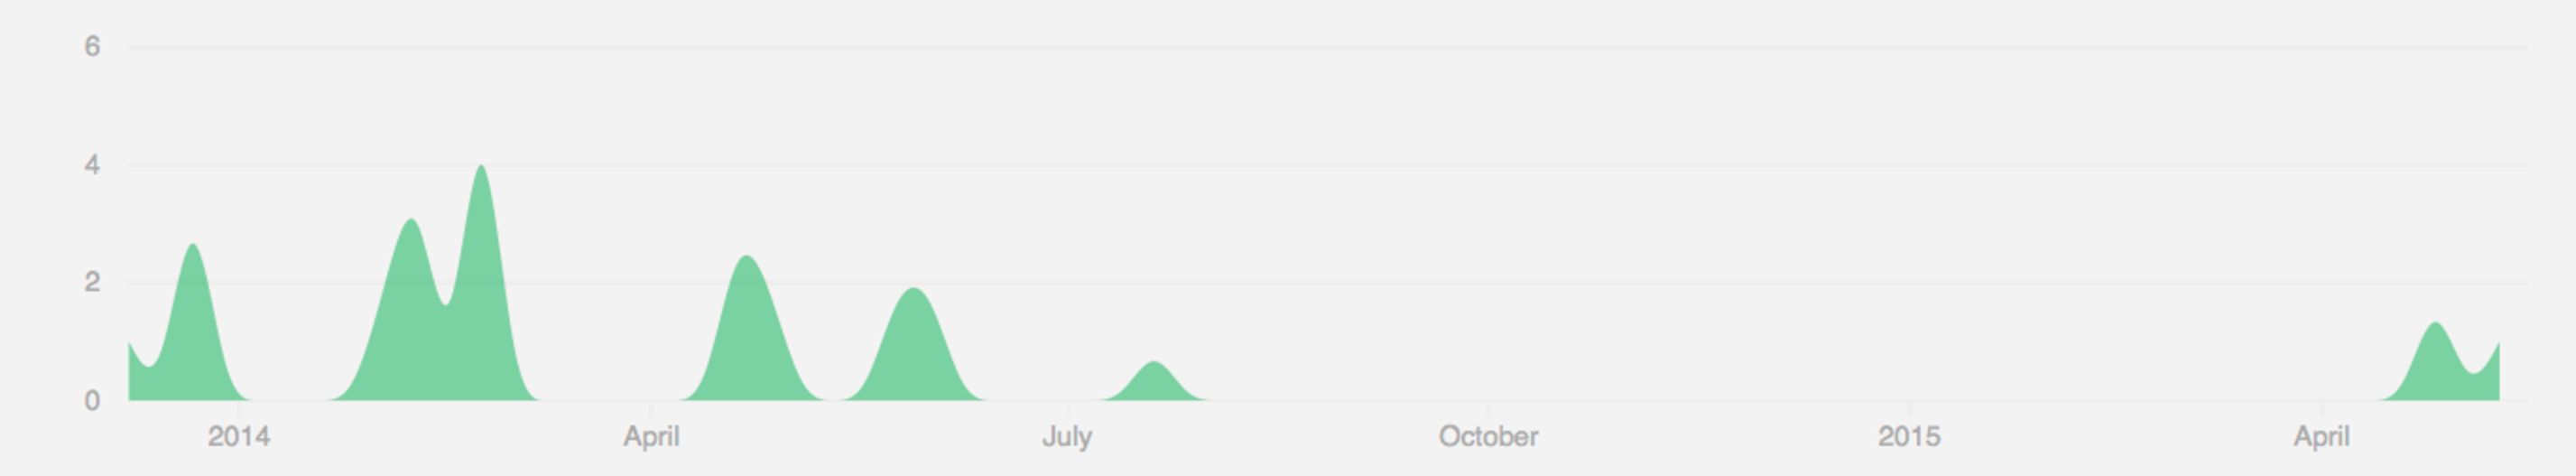
\includegraphics[width=1.0\linewidth]
{pictures/sites_contributions.pdf}
\caption{Commits contributed by CMS site admins to SiteInfoProvider tools repository}
\label{fig:github_stats}
\end{figure}

